\documentclass[12pt, a4paper]{article} %determina o tamanho da fonte, o tipo de papel e o tipo de documento.

\setlength{\parindent}{1.0 cm} %tamanho do espaço para começar o parágrafo.
\setlength{\parskip}{0.5cm} %tamanho do espaço entre os parágrafos.

%Aqui ficam os pacotes utilizados para formatação do documento de modo geral:

\usepackage[utf8]{inputenc} 
\usepackage{indentfirst} %Coloca espaços nos inícios de parágrafos automaticamente. 
\usepackage[brazilian]{babel} %
\usepackage{amsmath}
\usepackage[hmargin=3cm, vmargin=2.5cm, bmargin=2.5cm]{geometry}
\usepackage{multicol}
\usepackage{graphicx} %para poder inserir imagens
\usepackage{subfig}
\usepackage{booktabs} 
\usepackage{hyperref} %para poder adicionar links e hiperlinks
\usepackage{float} %para poder posicionar as imagens
\usepackage{subfig} %para colocar duas imagens juntas

\usepackage{listings} %para poder incluir códigos
\usepackage{xcolor}
\definecolor{codegreen}{rgb}{0,0.6,0}
\definecolor{codegray}{rgb}{0.5,0.5,0.5}
\definecolor{codepurple}{rgb}{0.58,0,0.82}
\definecolor{backcolour}{rgb}{0.95,0.95,0.92}
\lstdefinestyle{mystyle}{
    backgroundcolor=\color{backcolour},   
    commentstyle=\color{codegreen},
    keywordstyle=\color{magenta},
    numberstyle=\tiny\color{codegray},
    stringstyle=\color{codepurple},
    basicstyle=\ttfamily\footnotesize,
    breakatwhitespace=false,         
    breaklines=true,                 
    captionpos=b,                    
    keepspaces=true,                 
    numbers=left,                    
    numbersep=5pt,                  
    showspaces=false,                
    showstringspaces=false,
    showtabs=false,                  
    tabsize=2,
    morecomment={l}[!],
    language=[77]Fortran,
}
\lstset{style=mystyle}

\begin{document} %começa alguma coisa,neste caso, o documento, sempre importante lembrar de colocar o \end{} para não dar erro 
	
	\begin{titlepage}
		\begin{center}
\Huge{Universidade de São Paulo}\\
\large{Instituto de Física de São Carlos}\\
\vspace{20pt}
\vspace{200pt}
\textbf{Lista 4}\\
\vspace{8cm}
		\end{center}

\begin{flushleft}
\begin{tabbing}
Pedro Calligaris Delbem 5255417\\
\end{tabbing}
\vspace{0.5cm}
Professor: Attilio Cucchieri\\		
		\end{flushleft}
	
		\begin{center}
			\vspace{\fill}
	Junho de 2025	
		\end{center}
	\end{titlepage}

%####################################################################### SUMÁRIO
	\tableofcontents 
	\thispagestyle{empty}
	\newpage
%#########################################################################

\section{Matrix Operations}

    \subsection{Exerc\'icio 1}

        Tarefa: Considere a matriz $n \times n$:

        $$
        A = 
        \begin{pmatrix}
        -5/2 & 4/3 & -1/12 & 0 & \dots & 0 & 0 \\
        4/3 & -5/2 & 4/3 & -1/12 & \dots & 0 & 0 \\
        -1/12 & 4/3 & -5/2 & 4/3 & \dots & 0 & 0 \\
        0 & -1/12 & 4/3 & -5/2 & \dots & 0 & 0 \\
        \vdots & \vdots & \vdots & \vdots & \ddots & \vdots & \vdots \\
        0 & 0 & 0 & 0 & \dots & -5/2 & 4/3 \\
        0 & 0 & 0 & 0 & \dots & 4/3 & -5/2 
        \end{pmatrix}
        $$
        
        \begin{itemize}
            \item Use o método de Householder para obter a correspondente matriz tridiagonal $A_{t}$.
        
            \item Verifique o produto $A_{t} = O^{T}AO$.
        
            \item Calcule o menor e o maior autovalor $\lambda$, e os correspondentes autovetores $y_{t}$, de $A_{t}$.
        
            \item Calcule os correspondentes autovetores y de A.
        
            \item Verifique a equação $Ay = \lambda y$ para esses autovalores.
        
        \end{itemize}
        
        Considere os casos $n=10$ e $n=20$.
        
        O c\'odigo foi compilado com o comando:

gfortran -ffree-form -ffree-line-length-none L6-5255417-ex-1.f90 -Wall -Wextra -pedantic -o L6-5255417-ex-1.exe

        Resultados:

        Obteve-se os seguintes resultados:
        \begin{figure}[H]
            \centering
            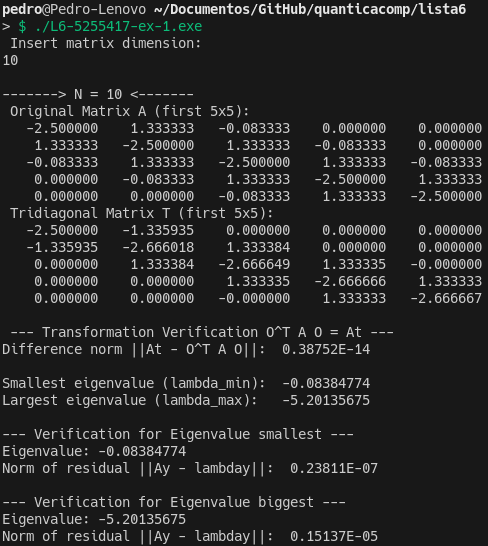
\includegraphics[width=0.8\textwidth]{../images/ex1-10.png}
        \end{figure}
        \begin{figure}[H]
            \centering
            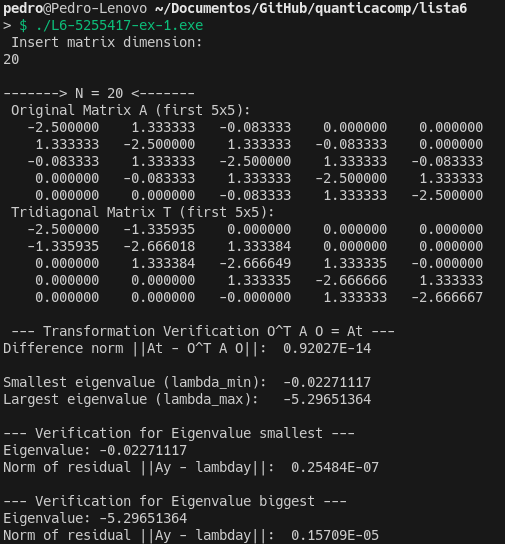
\includegraphics[width=0.8\textwidth]{../images/ex1-20.png}
        \end{figure}

        Nota-se que todas as verifica\c{c}\~oes resultaram em valores pequenos, mostrando que o m\'etodo funcionou bem para ambos os casos.
        (O c\'odigo gera dois arquivos - "At\_eingenvalues.txt" e "A\_eingenvalues.txt" - com os autovetores de $A_t$ e A - respectivamente - que n\~ao foram colocados no terminal para n\~ao poluir a vizualiza\c{c}\~ao dos resultados)


\end{document}